\setcounter{figure}{0}
\begin{questions}

\question Find the volume of the solid whose base is the region bounded by the semicircle $y=\sqrt{4-x^2}$ and the $x$-axis and whose cross sections through the solid perpendicular to the $x$-axis are squares. For a 3D graph, go to \url{https://sagecell.sagemath.org/?q=ixkvvn}.
\begin{figure}[hbt!]\centering
  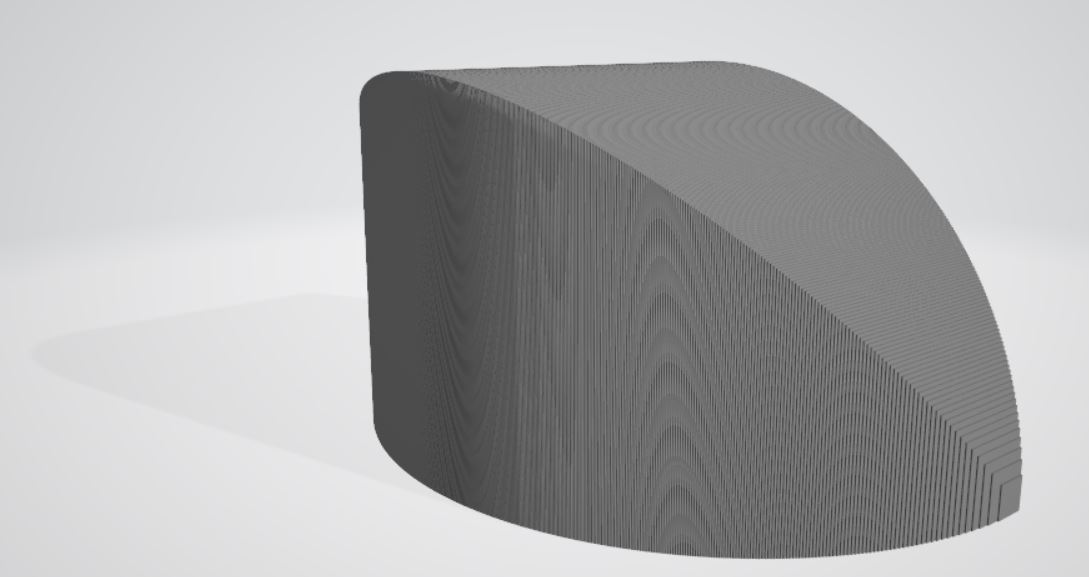
\includegraphics[scale=0.4]{plots/cross_section_squares.JPG}
  \caption{For a better view, go to \url{https://sagecell.sagemath.org/?q=rvlawp}.}
\end{figure}
\begin{solutionorbox}[6.0in]

\end{solutionorbox}

\newpage


\question Find the volume of the solid whose base is the region bounded by $y=x^2$ and the the line $y=4$ and whose cross sections are equilateral triangles parallel to the $x$-axis.
\begin{figure}[hbt!]\centering
  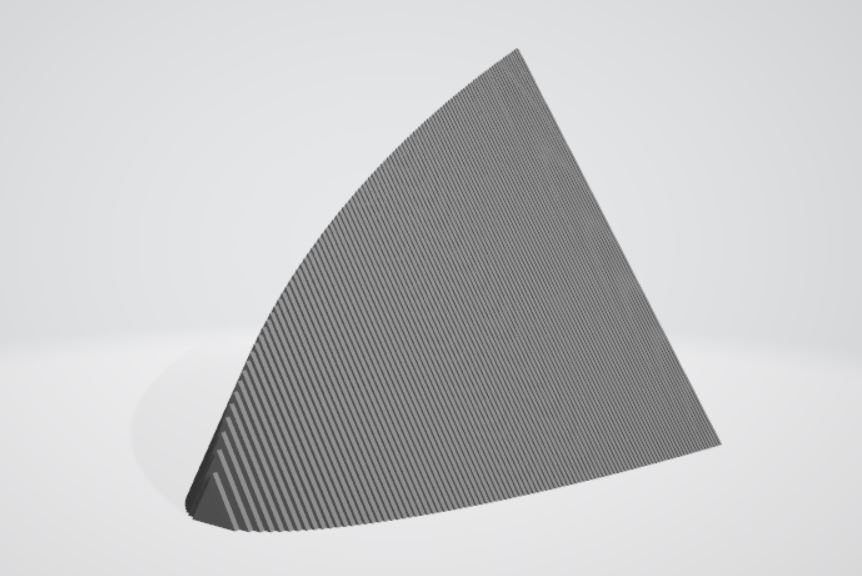
\includegraphics[scale=0.5]{plots/cross_section_triangles.JPG}
  \caption{For a better view, go to \url{https://sagecell.sagemath.org/?q=rvlawp}.}
\end{figure}

\begin{solutionorbox}[6.25in]

\end{solutionorbox}


\newpage


\question Let $R$ be the region bounded by the following curves. Use the disk (or washer) method to find the volume of the solid generated when $R$ is revolved about the $x$-axis.
\begin{parts}
\part $y=e^{-x}$ and the $x$-axis on the interval $[0,\ln(4)]$
  \begin{figure}[hbt!]\centering
    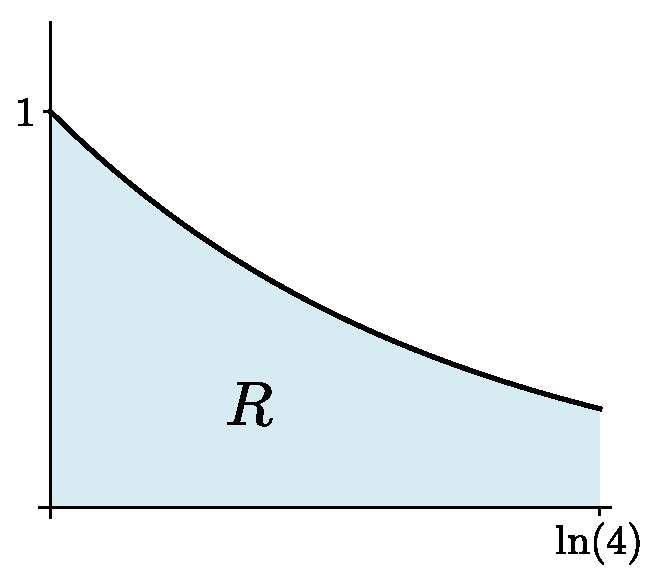
\includegraphics[scale=0.75]{plots/volumes_by_slicing_p1.pdf}
    \caption{Region bounded by $y=e^{-x}$ and the $x$-axis on the interval $[0, \,\ln(4)]$}
  \end{figure}

\begin{solutionorbox}[5.50in]

\end{solutionorbox}


\newpage


\part $y=x$ and $y=\sqrt[4]{x}$
  \begin{figure}[hbt!]\centering
    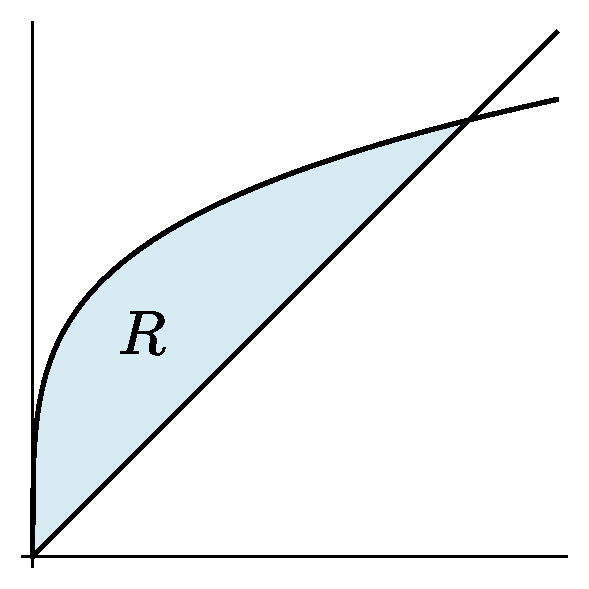
\includegraphics[scale=0.75]{plots/volumes_by_slicing_p2.pdf}
    \caption{Region bounded by $y=\sqrt[4]{x}$ and the $y=x$}
  \end{figure}

\begin{solutionorbox}[5.9in]

\end{solutionorbox}

\end{parts}


\newpage


\question Let $R$ be the region bounded by the following curves. Use the disk (or washer) method to find the volume of the solid generated when $R$ is revolved about the $y$-axis.
\begin{parts}

\part $y=16-x^2$ and the $x$-axis
  \begin{figure}[hbt!]\centering
    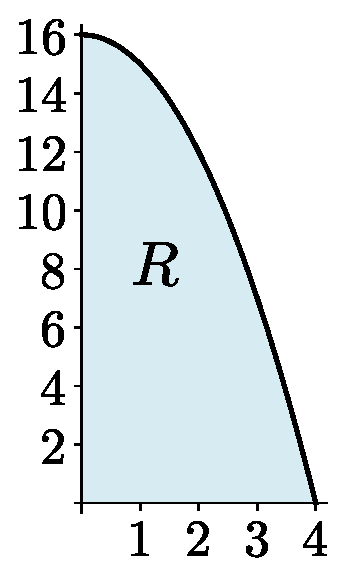
\includegraphics[scale=0.75]{plots/volumes_by_slicing_p4.pdf}
    \caption{Region bounded by $y=16-x^2$ and the $x$-axis}
  \end{figure}
  
\begin{solutionorbox}[5.4in]

\end{solutionorbox}

\newpage

\part $\displaystyle y=\frac{x}{2}$ and $y=\sqrt{x}$
  \begin{figure}[hbt!]\centering
    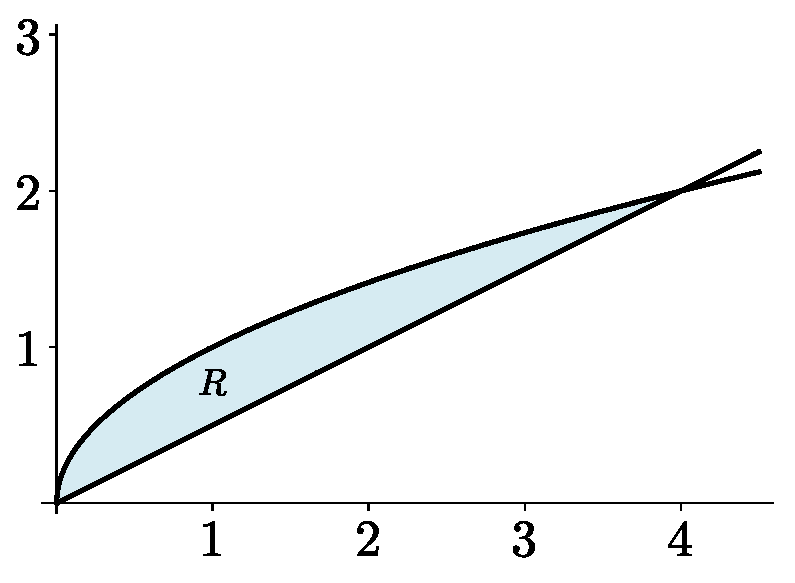
\includegraphics[scale=0.75]{plots/volumes_by_slicing_p5.pdf}
    \caption{Region bounded by $y=16-x^2$ and the $x$-axis}
  \end{figure}
  
\begin{solutionorbox}[6.00in]

\end{solutionorbox}

\end{parts}


\end{questions}